\documentclass[11pt,a4paper]{article}
\usepackage[margin=1in]{geometry}
\usepackage[T1]{fontenc}
\usepackage[utf8]{inputenc}
\usepackage{mathptmx}\usepackage[scaled=0.9]{helvet}
\usepackage{microtype}
\usepackage{booktabs}
\usepackage{enumitem}
\usepackage{xcolor}
\usepackage{tikz}
\usetikzlibrary{positioning,arrows.meta,fit,backgrounds,calc}
\usepackage{listings}
\usepackage{tcolorbox}
\usepackage{titlesec}
\usepackage{fancyhdr}
\usepackage{longtable}
\usepackage{array}
\newcolumntype{P}[1]{>{\raggedright\arraybackslash}p{#1}}
\usepackage[hidelinks]{hyperref}

\definecolor{mmblue}{HTML}{1F4E79}
\definecolor{mmorange}{HTML}{C55A11}
\definecolor{mmgreen}{HTML}{2E7D32}
\definecolor{mmgray}{HTML}{F2F2F2}
\definecolor{codebg}{HTML}{F7F7F7}

\titleformat{\section}{\Large\bfseries\color{mmblue}}{\thesection}{0.8em}{}
\titleformat{\subsection}{\large\bfseries\color{mmblue}}{\thesubsection}{0.8em}{}
\setlist{nosep}

\lstset{
  basicstyle=\ttfamily\small,
  backgroundcolor=\color{codebg},
  frame=single, rulecolor=\color{black!15},
  breaklines=true, columns=fullflexible, keepspaces=true,
  showstringspaces=false
}

\pagestyle{fancy}
\fancyhf{}
\lhead{\small Megamind --- Design Document}
\rhead{\small v0.1}
\cfoot{\small\thepage}

\newtcolorbox{decision}{colback=mmblue!5,colframe=mmblue,title=Decision,fonttitle=\bfseries,left=4pt,right=4pt,top=2pt,bottom=2pt}
\newtcolorbox{risk}{colback=mmorange!6,colframe=mmorange,title=Risk,fonttitle=\bfseries,left=4pt,right=4pt,top=2pt,bottom=2pt}

\title{\textbf{\color{mmblue}Megamind}\\[4pt]\large Egocentric Memory for Meta Quest 3: Design Document}
\author{Project lead: Devin \quad\textperiodcentered\quad Team: 4 engineers}
\date{v0.1 --- Hackathon build}

\begin{document}
\maketitle
\thispagestyle{empty}

\begin{abstract}
\noindent Megamind gives a Meta Quest 3 wearer an AI assistant that remembers what they have seen. The headset's passthrough cameras are sampled continuously; keyframes are filtered, described, embedded, and stored as \emph{memory tokens} in a vector database. A Claude-based agent exposes a \texttt{recall\_memory} tool; when invoked, relevant tokens are retrieved and handed to a Qwen vision-language ``reader'' sub-agent that attends over the concatenated tokens and returns grounded evidence. Claude composes the final answer, which is delivered through a voice-first AR chat interface on the headset. This document fixes the architecture, interfaces, model choices, work split and risk plan so that four engineers and several coding agents can build it in parallel.
\end{abstract}

\tableofcontents
\newpage

% -------------------------------------------------------------------
\section{Goals and Scope}

\subsection{Goal}
Demonstrate, live, a wearer asking the headset questions whose answers depend on things they saw earlier---``Where did I leave my keys?'', ``What was the name on that whiteboard?'', ``Who did I talk to after lunch?''---and receiving correct, grounded answers with a visual citation of the remembered moment.

\subsection{In scope}
\begin{itemize}
  \item Continuous passthrough capture on Quest~3, sampled and uploaded as keyframes.
  \item Server-side filtering, captioning/OCR, embedding and storage of memory tokens.
  \item A Claude agent with a \texttt{recall\_memory} tool; a Qwen-VL reader sub-agent that performs attention over retrieved tokens.
  \item Voice-first AR chat panel on the headset (push-to-talk in, text + speech out), with the cited memory thumbnail shown.
  \item A laptop/webcam feeder that emulates the headset so the backend is testable without hardware.
\end{itemize}

\subsection{Explicitly out of scope}
\begin{itemize}
  \item Training or fine-tuning any model; learned ``soft'' memory tokens.
  \item On-device inference. Everything heavy runs on the server.
  \item Multi-user memory, auth, or long-term privacy controls beyond a purge button.
  \item Quest 2 / Quest Pro support (no camera API).
\end{itemize}

% -------------------------------------------------------------------
\section{Prior Art and Differentiation}
The use case is not new; the open, agent-callable system on a consumer headset is. Details and links in \texttt{docs/prior-art.md}.

\paragraph{Products.} Google's \emph{Project Astra} (I/O 2024, now Gemini Live / Android XR) demonstrated ``where did I leave my glasses?'' from a short rolling window of camera frames---closed, session-scoped, no third-party access. Meta AI on Ray-Ban Meta offers explicit ``remember where I parked'' reminders and Live AI sessions, not passive searchable visual memory. Limitless, Rewind, Bee and Omi pendants are audio-only lifeloggers.

\paragraph{Research.} \emph{Ego4D Episodic Memory} (2022) defines our exact task (NLQ, Visual Queries) as an offline benchmark. \emph{EgoLife} (CVPR 2025) is the closest system: a week-long egocentric assistant with EgoRAG, a caption/text-based hierarchical memory, captured on Aria glasses with no interactive AR client. \emph{Vinci} (2024) is a real-time egocentric VLM assistant for smart glasses focused on live understanding.

\paragraph{Open source on Quest.} \texttt{QuestCameraKit} ($\sim$580$\star$) provides Passthrough Camera API templates (reuse its plumbing). \texttt{JarvisVR}, \texttt{OpenAI-for-Meta-Quest-3} and similar projects answer questions about the \emph{current} scene; JarvisVR explicitly lists episodic memory as future work.

\paragraph{What Megamind adds.}
\begin{enumerate}
  \item Persistent, passive episodic \emph{visual} memory on a consumer headset via the Passthrough Camera API.
  \item Memory exposed as an agent tool (\texttt{recall\_memory}) with a published schema, decoupled from any one assistant.
  \item A two-model read path in which a Qwen-VL reader re-attends over the retrieved \emph{frames}, not just captions.
  \item Temporal + semantic + visual hybrid retrieval with time-range filtering.
  \item Grounded answers: the cited frame is rendered in AR next to the reply.
  \item Open, device-agnostic (feeder, phone, webcam) with a local-first store and purge.
\end{enumerate}
We claim a working, open, agent-integrated system on hardware people own---not a new use case or a model-level contribution.

% -------------------------------------------------------------------
\section{Key Design Decisions}

\begin{decision}
\textbf{D1 --- One Unity app on the headset does both capture and chat.}
Horizon OS keeps a single immersive app in the foreground and suspends others, so a separate chat app or WebXR page would stop capture. Streams~1 and~3 therefore share one Android APK.
\end{decision}

\begin{decision}
\textbf{D2 --- A memory token is a record, not a learned vector.}
Each token = one keyframe at time $t$ with: a dense caption, OCR text, entity list, a text embedding, an image embedding, and the JPEG thumbnail. ``Attention over tokens'' is performed by the Qwen-VL reader, which receives the concatenated captions \emph{and} thumbnails as real vision/text tokens in its context. This is honest to the pitch and buildable in a day.
\end{decision}

\begin{decision}
\textbf{D3 --- Two-model agent: Claude orchestrates, Qwen-VL reads memory.}
Claude (Sonnet) is the user-facing agent and tool caller. The \texttt{recall\_memory} tool retrieves top-$k$ tokens and invokes a Qwen2.5-VL (or Qwen3-VL) reader that answers the sub-question over those tokens with citations. Claude never sees raw frames unless the reader's evidence is insufficient, keeping its context small and latency bounded.
\end{decision}

\begin{decision}
\textbf{D4 --- All intelligence is server-side; the headset is a thin client.}
The headset uploads JPEG keyframes and audio, and renders text/audio/thumbnails. Every server endpoint is exercisable with \texttt{curl}, so backend progress never waits on a headset build.
\end{decision}

\begin{decision}
\textbf{D5 --- LanceDB as the memory store.}
Embedded, pip-installable, supports vector + full-text + metadata filtering. No Docker, no infra. Wrapped behind a \texttt{MemoryStore} interface so it can be swapped for pgvector/Qdrant if needed.
\end{decision}

\begin{decision}
\textbf{D6 --- Voice first.}
Push-to-talk (controller button or hand pinch) $\rightarrow$ server STT. Replies are spoken (server TTS) and shown on a world-locked panel. Typing in VR is not supported.
\end{decision}

% -------------------------------------------------------------------
\section{System Architecture}

\begin{figure}[h]
\centering
\resizebox{\textwidth}{!}{%
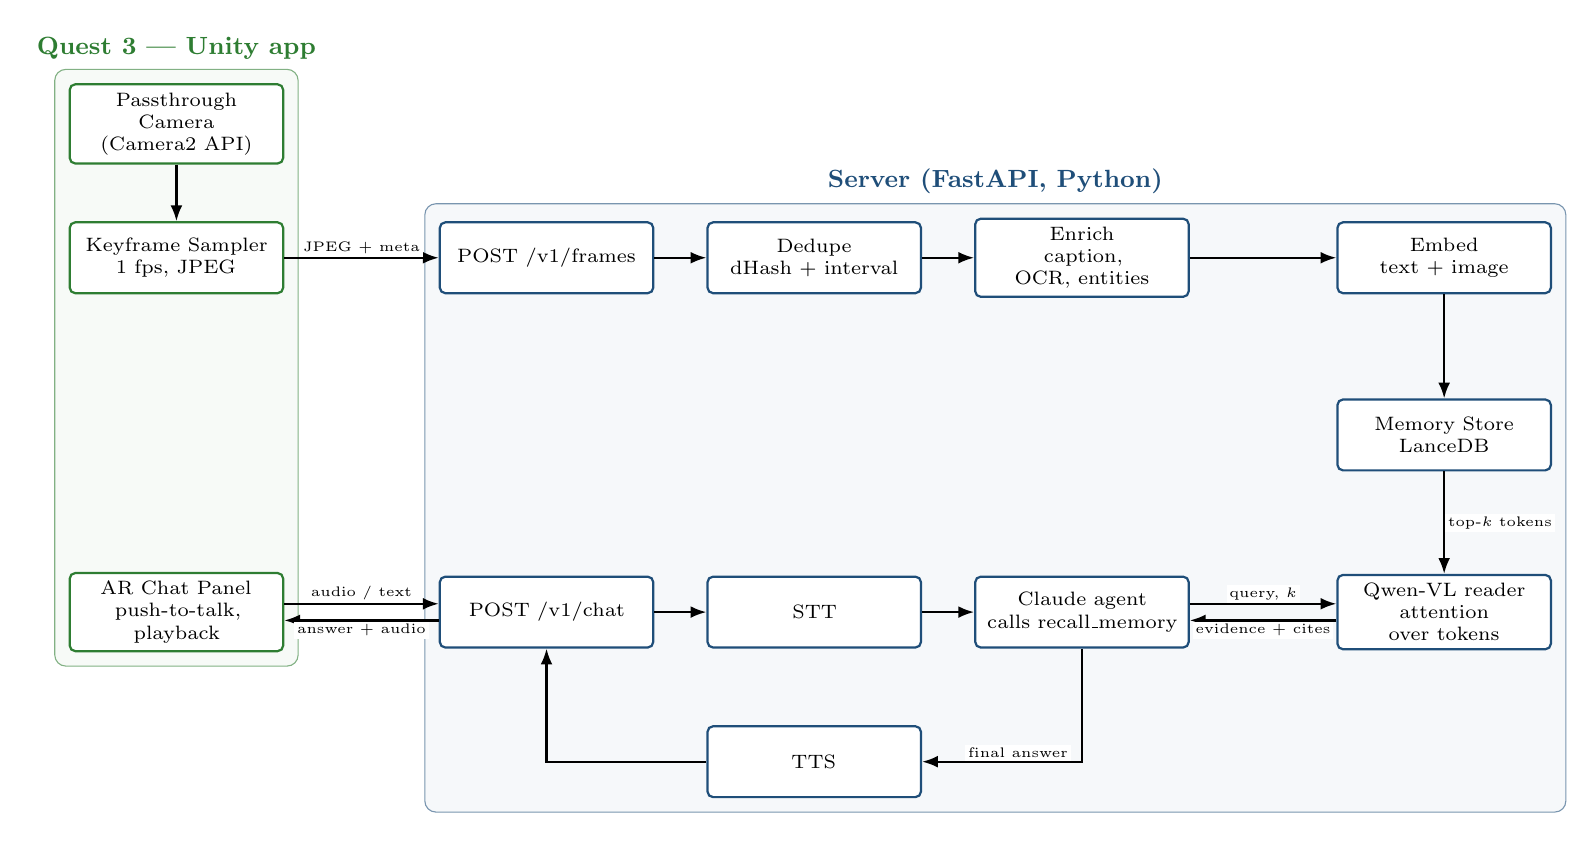
\begin{tikzpicture}[
  box/.style={draw, rounded corners=2pt, align=center, minimum height=9mm, minimum width=26mm, text width=25mm, inner sep=3pt, font=\scriptsize, fill=white},
  hs/.style={box, draw=mmgreen, thick},
  sv/.style={box, draw=mmblue, thick},
  arr/.style={-{Latex[length=2mm]}, thick},
  lbl/.style={font=\tiny, fill=white, inner sep=1pt}
]
% Headset column
\node[hs] (cam) at (0.9,1.7) {Passthrough Camera\\(Camera2 API)};
\node[hs] (sampler) at (0.9,0) {Keyframe Sampler\\1 fps, JPEG};
\node[hs] (ui) at (0.9,-4.5) {AR Chat Panel\\push-to-talk, playback};
% Server ingest row
\node[sv] (frames) at (5.6,0) {POST /v1/frames};
\node[sv] (dedupe) at (9.0,0) {Dedupe\\dHash + interval};
\node[sv] (enrich) at (12.4,0) {Enrich\\caption, OCR, entities};
\node[sv] (embed) at (17.0,0) {Embed\\text + image};
\node[sv] (store) at (17.0,-2.25) {Memory Store\\LanceDB};
% Server agent row
\node[sv] (chat) at (5.6,-4.5) {POST /v1/chat};
\node[sv] (stt) at (9.0,-4.5) {STT};
\node[sv] (claude) at (12.4,-4.5) {Claude agent\\calls recall\_memory};
\node[sv] (reader) at (17.0,-4.5) {Qwen-VL reader\\attention over tokens};
\node[sv] (tts) at (9.0,-6.4) {TTS};
\begin{scope}[on background layer]
\node[fit=(cam)(sampler)(ui), draw=mmgreen!60, fill=mmgreen!4, rounded corners, inner sep=5pt, label={[font=\small\bfseries\color{mmgreen}]above:Quest 3 --- Unity app}] {};
\node[fit=(frames)(dedupe)(enrich)(embed)(store)(chat)(stt)(claude)(reader)(tts), draw=mmblue!60, fill=mmblue!4, rounded corners, inner sep=5pt, label={[font=\small\bfseries\color{mmblue}]above:Server (FastAPI, Python)}] {};
\end{scope}
% arrows
\draw[arr] (cam) -- (sampler);
\draw[arr] (sampler) -- node[lbl, above]{JPEG + meta} (frames);
\draw[arr] (frames) -- (dedupe);
\draw[arr] (dedupe) -- (enrich);
\draw[arr] (enrich) -- (embed);
\draw[arr] (embed) -- (store);
\draw[arr, transform canvas={yshift=3pt}] (ui) -- node[lbl, above]{audio / text} (chat);
\draw[arr, transform canvas={yshift=-3pt}] (chat) -- node[lbl, below]{answer + audio} (ui);
\draw[arr] (chat) -- (stt);
\draw[arr] (stt) -- (claude);
\draw[arr, transform canvas={yshift=3pt}] (claude) -- node[lbl, above]{query, $k$} (reader);
\draw[arr, transform canvas={yshift=-3pt}] (reader) -- node[lbl, below]{evidence + cites} (claude);
\draw[arr] (store) -- node[lbl, right]{top-$k$ tokens} (reader);
\draw[arr] (claude) |- node[lbl, pos=0.7, above]{final answer} (tts);
\draw[arr] (tts) -| (chat);
\end{tikzpicture}}
\caption{End-to-end data flow. Green: headset. Blue: server. Top row is Stream 1 (ingest); bottom rows are Streams 2--3 (agent and chat).}
\end{figure}

\subsection{Components}
\begin{description}[style=nextline]
  \item[Headset app (Unity 2022.3 LTS / Unity 6, Meta XR SDK $\geq$ v74).] Reads the passthrough camera via Meta's Passthrough Camera API (exposed as Android Camera2; the Meta sample wraps it in \texttt{WebCamTextureManager}). Samples one frame per second, encodes JPEG ($\leq$ 960 px wide, quality 75), and POSTs to \texttt{/v1/frames} with device id, UTC timestamp and head pose. Renders a world-locked chat panel; records microphone on push-to-talk; plays returned audio.
  \item[Ingest service (\texttt{server/megamind/ingest}).] Accepts frames, drops near-duplicates (perceptual dHash Hamming distance $<$ 6 within the last 30 s, and minimum 2 s gap), then enqueues to a worker that produces a memory token (Section~\ref{sec:token}) and writes it to the store.
  \item[Memory store (\texttt{server/megamind/store}).] LanceDB table of memory tokens with two vector columns (text, image) and full-text search on \texttt{caption} + \texttt{ocr\_text}. Hybrid query: vector + BM25 fused by reciprocal rank, pre-filtered by time range.
  \item[Agent service (\texttt{server/megamind/agent}).] STT $\rightarrow$ Claude with tools $\rightarrow$ (\texttt{recall\_memory} $\rightarrow$ store $\rightarrow$ Qwen-VL reader) $\rightarrow$ Claude answer $\rightarrow$ TTS. Returns text, audio, and the ids/thumbnails of memories cited.
  \item[Feeder (\texttt{tools/feeder.py}).] Emulates the headset from a laptop webcam or a video file. Used for all backend development and as a demo fallback.
\end{description}

% -------------------------------------------------------------------
\section{Stream 1 --- Vision Capture and Memory Tokenization}

\subsection{Capture on Quest 3}
\begin{itemize}
  \item Requires Quest 3 / 3S on Horizon OS v74+ with developer mode. Android manifest needs \texttt{horizonos.permission.HEADSET\_CAMERA} and \texttt{android.permission.CAMERA}; the user grants it at runtime.
  \item Use the \texttt{PassthroughCameraApiSamples} pattern: \texttt{WebCamTextureManager} selects the left RGB camera, max 1280$\times$960 @ 30 fps. We read \texttt{WebCamTexture} into a \texttt{Texture2D} once per second, downscale to 960 px wide and \texttt{EncodeToJPG(75)}.
  \item Upload with \texttt{UnityWebRequest} multipart POST, fire-and-forget with a bounded queue (drop oldest if $>$ 10 pending). Target $\sim$80--120 KB/frame, $\sim$1 Mbit/s.
  \item Also send head pose (position + yaw) from \texttt{OVRCameraRig}; it is cheap and enables ``where'' answers later.
  \item Do not attempt video streaming or on-device inference.
\end{itemize}

\subsection{Filtering}
Two-stage, deliberately simple:
\begin{enumerate}
  \item \textbf{Client:} fixed 1 fps sample.
  \item \textbf{Server:} dHash (8$\times$8) against the last 30 s of accepted frames; reject if Hamming distance $<$ 6. Enforce a 2 s minimum gap. Reject frames with mean luminance $<$ 20 (lens covered/dark). Expected keep rate 10--30\%.
\end{enumerate}

\subsection{Memory token}\label{sec:token}
\begin{lstlisting}
MemoryToken {
  id:             str   # ulid
  device_id:      str
  ts:             float # unix seconds, UTC
  caption:        str   # 1-3 dense sentences from the VLM
  ocr_text:       str   # any legible text, verbatim
  entities:       list[str]   # objects, people descriptors, places
  pose:           {x,y,z,yaw} | null
  text_vec:       float[1024] # embedding of caption + ocr + entities
  image_vec:      float[768]  # SigLIP image embedding
  thumb_path:     str   # JPEG on disk, served at /v1/thumbs/{id}.jpg
  frame_hash:     str   # dHash hex
  episode_id:     str | null  # filled by consolidation (stretch)
}
\end{lstlisting}

\paragraph{Enrichment model.} Qwen2.5-VL-7B-Instruct (or Qwen3-VL) via an OpenAI-compatible endpoint (vLLM locally if a GPU is available, otherwise a hosted provider). One call per keyframe with a fixed JSON-output prompt producing \texttt{caption}, \texttt{ocr\_text}, \texttt{entities}. Fallback: Claude Haiku with vision. Prompt emphasises \emph{retrievable} detail: object locations relative to surfaces, legible text verbatim, people descriptors (no identity claims), room type.

\paragraph{Embeddings.} Text: a hosted embedding model (Voyage \texttt{voyage-3} or OpenAI \texttt{text-embedding-3-small}) or local \texttt{bge-m3}. Image: SigLIP-base (\texttt{open\_clip}) for visual-similarity queries. Both configurable via environment variables.

\paragraph{Consolidation (stretch).} Every 10 minutes, summarise accepted tokens into an \emph{episode} token (``10:05--10:15: in the kitchen, made coffee, phone on counter'') to help vague queries. Optional.

\begin{risk}
Camera API bring-up is the single largest risk: SDK/OS version mismatch, permission not granted, \texttt{WebCamTexture} returning black. Mitigation: hour-0 spike using Meta's sample scene unchanged before any custom code; feeder as fallback for every other stream.
\end{risk}

% -------------------------------------------------------------------
\section{Stream 2 --- Memory Retrieval and the Reader Sub-Agent}

\subsection{Tool interface exposed to Claude}
\begin{lstlisting}
recall_memory(
  query: str,              # natural-language description of what to find
  time_from: str | null,   # ISO-8601; null = no lower bound
  time_to:   str | null,
  k: int = 12,             # tokens to retrieve
  mode: "semantic" | "visual" | "hybrid" = "hybrid"
) -> {
  evidence:    str,        # reader's grounded answer to `query`
  confidence:  "high" | "medium" | "low" | "not_found",
  cited:       [{id, ts, caption, thumb_url}],
  all_retrieved: [{id, ts, caption}]
}
\end{lstlisting}
Claude's system prompt instructs it to call \texttt{recall\_memory} whenever the user's question references past perception, to translate relative times (``this morning'', ``ten minutes ago'') into absolute ISO ranges using the injected current time, and to answer ``I don't have a memory of that'' when confidence is \texttt{not\_found} rather than guess.

\subsection{Retrieval}
\begin{enumerate}
  \item Pre-filter by \texttt{ts} range (if any) and device.
  \item Hybrid search: cosine on \texttt{text\_vec} (query embedding) $+$ BM25 on caption/OCR, fused with RRF. In \texttt{visual} mode, embed the query with SigLIP's text tower and search \texttt{image\_vec}. \texttt{hybrid} unions both.
  \item Recency tie-break: among near-equal scores prefer newer.
  \item Return top-$k$ (default 12; hard cap 24 to bound reader cost).
\end{enumerate}

\subsection{Reader sub-agent (Qwen-VL)}
The reader receives, in one prompt, the concatenated tokens: for each, \texttt{[id] [timestamp] caption / ocr} plus the thumbnail image, followed by the query. It is asked to answer only from the tokens, cite token ids, and emit a confidence label as JSON. This is the component that literally performs attention across memories. Qwen2.5-VL-7B handles 12--24 images comfortably; use 72B via a hosted provider if quality is lacking.

\paragraph{Why two models.} Claude keeps the conversation, tool-use discipline and final phrasing; the reader does cheap, parallelisable, image-heavy evidence extraction. Claude's context never fills with thumbnails, so multi-turn chat remains fast.

\subsection{Latency budget (target $\leq$ 8 s to first spoken word)}
\begin{center}
\begin{tabular}{lr}
\toprule
STT (Whisper / Deepgram) & 0.8 s \\
Claude turn 1 (decide tool call) & 1.5 s \\
Retrieval (LanceDB) & 0.1 s \\
Reader (Qwen-VL, 12 images) & 2.5 s \\
Claude turn 2 (compose answer) & 1.5 s \\
TTS (first chunk) & 0.8 s \\
\midrule
Total & $\approx$ 7.2 s \\
\bottomrule
\end{tabular}
\end{center}
Stream Claude's final text to the panel while TTS renders so the UI feels responsive.

% -------------------------------------------------------------------
\section{Stream 3 --- AR Chat Interface}

\begin{itemize}
  \item \textbf{Scene:} \texttt{OVRCameraRig} with Passthrough enabled (Building Block), a world-locked \texttt{Canvas} panel 0.6 m wide placed 1 m ahead on first use and re-anchorable by a controller gesture.
  \item \textbf{Input:} push-to-talk on controller trigger (hand-tracking pinch as a stretch). Unity \texttt{Microphone} $\rightarrow$ 16 kHz mono WAV $\rightarrow$ \texttt{POST /v1/chat} (multipart). A ``listening'' indicator shows on the panel.
  \item \textbf{Output:} transcript bubbles (user/assistant), cited memory thumbnails rendered beside the assistant bubble (fetched from \texttt{thumb\_url}), audio played via \texttt{AudioSource} from the returned WAV URL.
  \item \textbf{Status HUD:} small indicator of capture state (frames/min accepted) and server connectivity.
  \item \textbf{Networking:} server reached over Tailscale (plain HTTP on the tailnet, \texttt{usesCleartextTraffic=true}) or an HTTPS ngrok tunnel. Base URL in a \texttt{ScriptableObject} config, overridable via a settings panel.
\end{itemize}

% -------------------------------------------------------------------
\section{API Contract}
All endpoints are JSON unless noted. Base path \texttt{/v1}. Authoritative version: \texttt{docs/api.md} in the repo.

\begin{longtable}{P{0.27\textwidth}P{0.68\textwidth}}
\toprule
\textbf{Endpoint} & \textbf{Description} \\
\midrule
\endhead
\texttt{GET /health} & \texttt{\{status, store\_count, models\}} \\
\texttt{POST /frames} & multipart: \texttt{image} (JPEG), \texttt{meta} JSON \texttt{\{device\_id, ts, pose?\}}. Returns \texttt{202 \{frame\_id, accepted, reason\}}. Non-blocking; enrichment is async. \\
\texttt{GET /memories} & Debug search. Query params \texttt{q, from, to, k, mode}. Returns tokens without vectors. \\
\texttt{GET /thumbs/\{id\}.jpg} & Keyframe thumbnail. \\
\texttt{POST /chat} & multipart or JSON: \texttt{session\_id}, and either \texttt{text} or \texttt{audio} (WAV). Returns \texttt{\{transcript, answer, audio\_url, cited:[\{id,ts,caption,thumb\_url\}], tool\_calls\}}. \\
\texttt{GET /audio/\{id\}.wav} & TTS output. \\
\texttt{DELETE /memories} & Purge all memory for a device (privacy / demo reset). \\
\bottomrule
\end{longtable}

% -------------------------------------------------------------------
\section{Repository Layout}
\begin{lstlisting}
megamind/
  README.md
  docs/
    megamind-design.tex / .pdf     # this document
    api.md                         # authoritative API contract
  server/                          # Python 3.11, FastAPI, uv/pip
    pyproject.toml
    megamind/
      main.py                      # app factory, routers
      config.py                    # env-driven settings
      models.py                    # pydantic schemas (MemoryToken, ...)
      ingest/   {router.py, filter.py, enrich.py, worker.py}
      store/    {base.py, lancedb_store.py}
      agent/    {router.py, claude_agent.py, reader.py, stt.py, tts.py, tools.py}
    tests/
  tools/
    feeder.py                      # webcam/video -> /v1/frames
    ask.py                         # CLI chat client
  headset/
    README.md                      # Unity project setup steps
    Megamind/                      # Unity project (committed sans Library/)
      Assets/Megamind/Scripts/{FrameUploader.cs, ChatClient.cs, ChatPanel.cs, ...}
\end{lstlisting}

% -------------------------------------------------------------------
\section{Work Split and Coordination}

\begin{center}
\begin{tabular}{P{0.22\textwidth}P{0.48\textwidth}P{0.24\textwidth}}
\toprule
\textbf{Owner} & \textbf{Scope} & \textbf{Agent support} \\
\midrule
Engineer 1 --- Headset capture & Unity project, Passthrough Camera bring-up, \texttt{FrameUploader.cs}, manifest/permissions, APK builds & Devin writes C\#, cannot run on device \\
Engineer 2 --- Headset UI/voice & Chat panel, push-to-talk, audio playback, thumbnails, config & Devin writes C\# \\
Engineer 3 --- Ingest + store & Reviews/tests agent-built ingest service with feeder; tunes filter and caption prompt & Devin agent builds end-to-end \\
Engineer 4 --- Agent + demo & Reviews/tests agent-built agent service; writes demo script; records fallback video & Devin agent builds end-to-end \\
Devin (lead) & API contract, repo skeleton, integration, agent coordination, unblocking & --- \\
\bottomrule
\end{tabular}
\end{center}

\paragraph{Integration rule.} Headset and server only communicate through \texttt{docs/api.md}. Any change to the contract is a PR that updates \texttt{api.md}, the pydantic models and the C\# DTOs together.

\paragraph{Phased plan.}
\begin{enumerate}
  \item \textbf{Hours 0--3: de-risk.} Camera sample runs on headset (E1). Repo skeleton + \texttt{/health} + feeder merged (Devin). Model API keys verified.
  \item \textbf{Hours 3--12: vertical slice.} Feeder $\rightarrow$ ingest $\rightarrow$ store $\rightarrow$ \texttt{GET /memories} works. \texttt{POST /chat} with text answers a question about feeder frames. Headset uploads real frames.
  \item \textbf{Hours 12--24: full loop.} Voice in/out on headset, thumbnails on panel, reader sub-agent live. First end-to-end ``where are my keys'' on hardware.
  \item \textbf{Final hours: demo hardening.} Fixed demo script, prompt tuning, latency trims, purge/reset, fallback video.
\end{enumerate}

% -------------------------------------------------------------------
\section{Risks and Mitigations}
\begin{center}
\begin{tabular}{P{0.34\textwidth}P{0.08\textwidth}P{0.5\textwidth}}
\toprule
\textbf{Risk} & \textbf{Sev.} & \textbf{Mitigation} \\
\midrule
Passthrough Camera API fails to deliver frames & High & Hour-0 spike with Meta sample; feeder fallback; phone camera as backup capture device \\
Unity build loop too slow & High & Thin client; all logic server-side and curl-testable; one build engineer only \\
Reader/VLM provider latency or outages & Med & Pluggable OpenAI-compatible endpoint; Claude Haiku vision fallback \\
Poor recall on demo queries & Med & Script the demo; tune caption prompt for object placement + OCR; hybrid search with time filter \\
Network from headset to laptop & Med & Tailscale on both; ngrok as backup; base URL editable at runtime \\
Scope creep (``real'' memory tokens, consolidation) & Med & Stretch goals gated behind a working demo \\
Privacy of bystanders & Low (hackathon) & Visible capture indicator, local storage, purge endpoint, no identity recognition in prompts \\
\bottomrule
\end{tabular}
\end{center}

% -------------------------------------------------------------------
\section{Configuration}
All secrets and model selections via environment variables (\texttt{server/.env.example}):
\begin{lstlisting}
ANTHROPIC_API_KEY=...
CLAUDE_MODEL=claude-sonnet-4-5
READER_BASE_URL=http://localhost:8001/v1      # vLLM or hosted OpenAI-compatible
READER_API_KEY=...
READER_MODEL=Qwen/Qwen2.5-VL-7B-Instruct
ENRICH_BASE_URL=${READER_BASE_URL}            # same model by default
EMBED_PROVIDER=openai|voyage|local
EMBED_MODEL=text-embedding-3-small
STT_PROVIDER=openai|deepgram
TTS_PROVIDER=openai|elevenlabs
LANCEDB_PATH=./data/lancedb
THUMB_DIR=./data/thumbs
\end{lstlisting}

\section{Open Questions}
\begin{itemize}
  \item GPU availability for local Qwen-VL via vLLM, or hosted only?
  \item Hackathon end time (fixes the phase boundaries above).
  \item Preferred STT/TTS vendor given available credits.
\end{itemize}

\end{document}
